\section{Valgrind}
Valgrind regroupe des outils d'analyse \textbf{dynamique}. L'analyse se fait en exécutant le programme.
% ----------
\subsection{Outils offerts par Valgrind}
\begin{itemize}
    \item Memcheck : Détection d'erreur mémoire (accès à de la mémoire non-allouée, valeurs non initialisées, double free, memcpy, fuites).
    \item Cachegrind : Profiler de mémoire cache (hit et miss), va aider à faire des programmes ayant un temps d'exécution plus rapide.
    \item Callgrind : Profiler de cache, à utiliser en complément de Cachegrind.
    \item Helgrind : Pour la détection d'erreur de thread dans des programmes multithreading. Aide à la programmation pour du multithread. (p.ex. problèmes liés l'absence de mutex.)
    \item DRD : idem helgrind
    \item Massif : Profiler de heap et stack (mémoire restante, fuites). Aide à faire des programmes moins gourmands en mémoires. Heap (Tas) grow from the bottom RAM, Stack (Pile) from the top.
    \item DHAT : Profiler de bloc dans le heap
\end{itemize}
% ----------
\subsection{Utilisation des outils}

\begin{figure}[H]
    \centering
    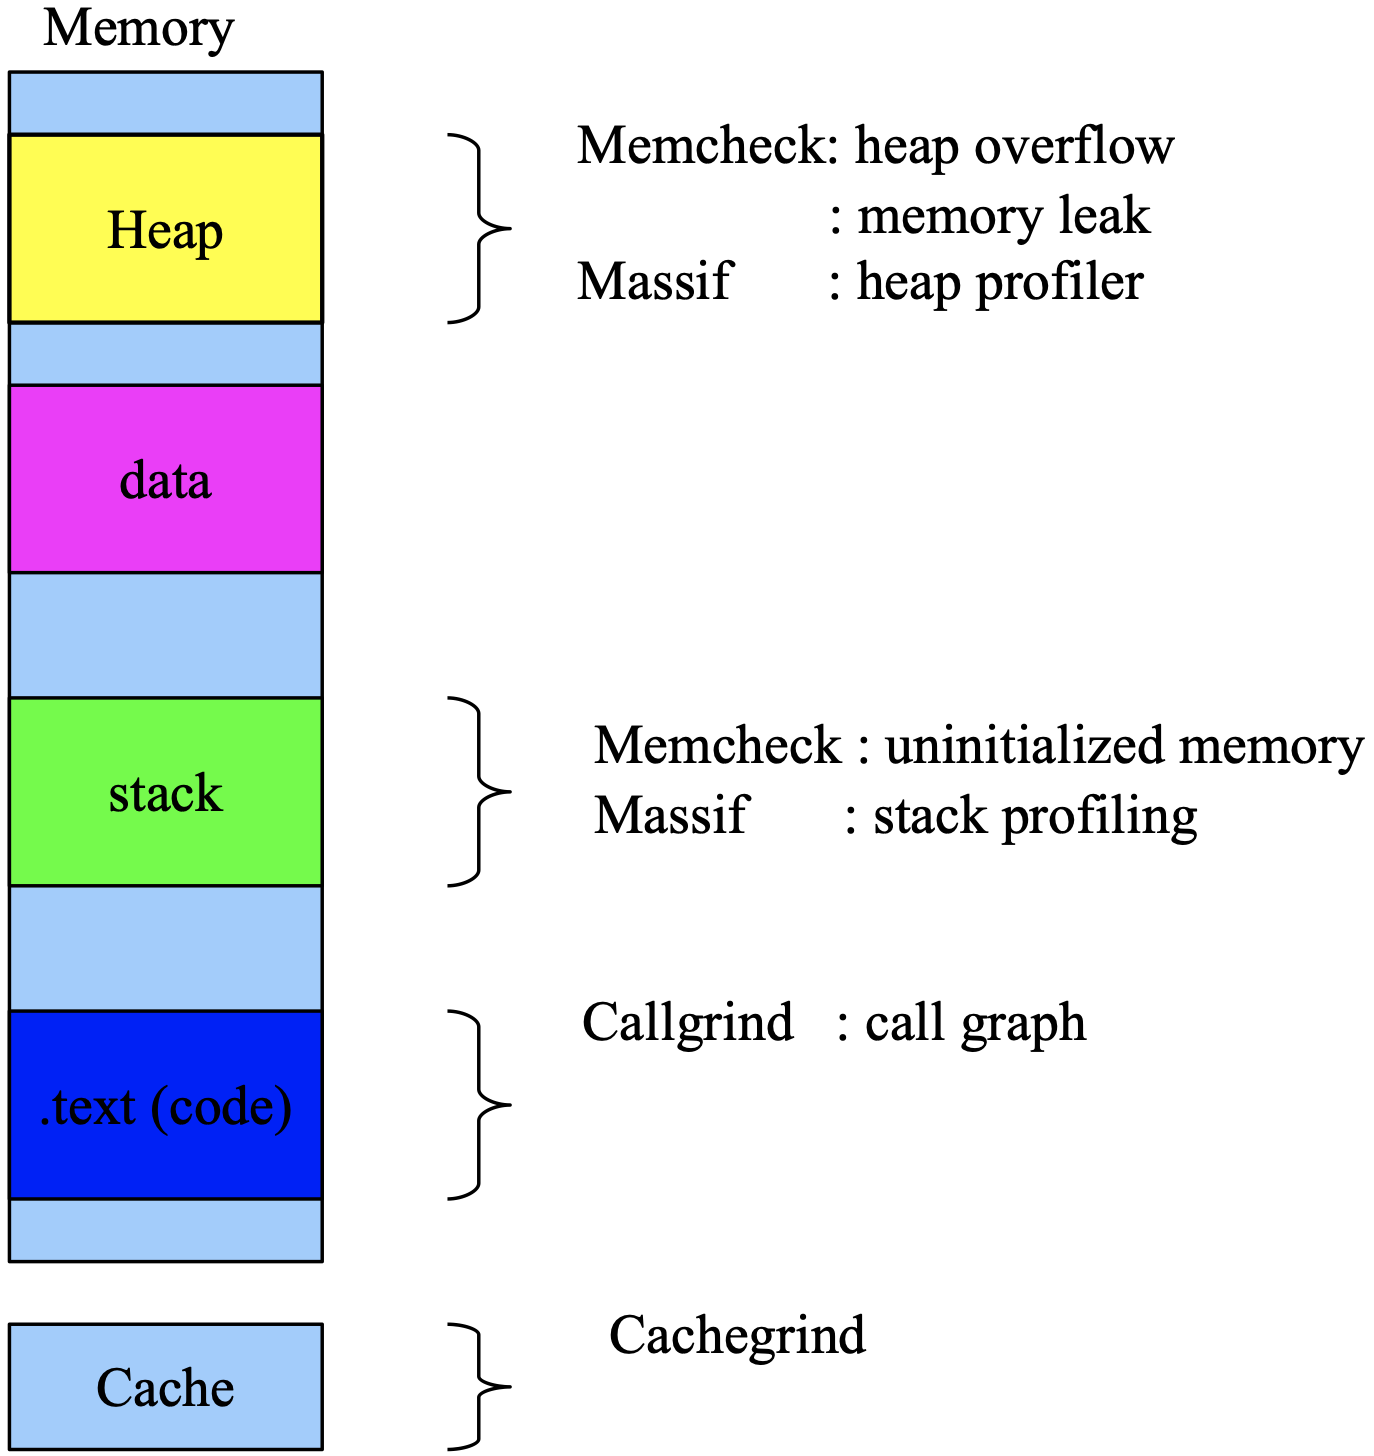
\includegraphics[width=.8\linewidth, angle=90]{valgrind_summary.png}
\end{figure}
%\begin{figure}[H]
%    \centering
%    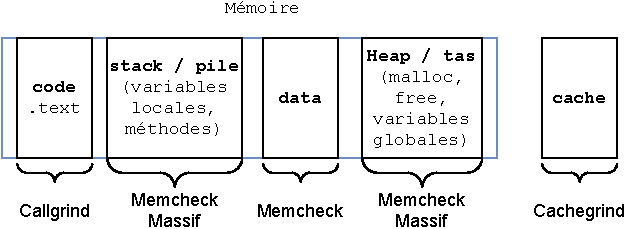
\includegraphics[width=0.6\columnwidth]{valgrind.pdf}
%\end{figure}

